% kuleuventheme2 by Janez Kren, September 2017, janez.kren@kuleuven.be, based on:
% kuleuventheme 1.3 by Roland Pastorino, 2013 roland.pastorino@kuleuven.be / www.rolandpastorino.com

\documentclass[11pt,t]{beamer}
\usetheme{kuleuven2}	%THEME OPTIONS for LOGO: kul (default), kulak, lrd,    ; OPTIONS for TITLE PAGE: normal (default), sedes


%%% OTHER SETTINGS
\usefonttheme[onlymath]{serif}			% math font with serifs, delete to make it sans-serif
\setbeamertemplate{footline}[body] 		% delete this line to remove footline bar on all frames
%\usepackage[orientation=landscape,size=custom,width=16,height=9,scale=0.5,debug]{beamerposter} %enable for widescreen 16:9 ratio
%\titlegraphic{ \includegraphics[width=.2\paperwidth]{mytitlepagepic.png} } %optional title page image


%%% ADDED PACKAGES:
\usepackage[english]{babel}
\usepackage{amsfonts}
\usepackage{amssymb}
\usepackage{amsmath}
\usepackage{subcaption}
\usepackage{algorithm2e}
\usepackage{setspace}
\usepackage{multirow}


%%% TITLE PAGE INFO:
\title[Avoiding local minima in Deep Learning]{Avoiding local minima in Deep Learning: a nonlinear optimal control approach} %[]] will appear in footline
\subtitle{Master's Thesis defence}

\author{Jan Scheers \\
Supervisor: Prof. dr. ir. Panos Patrinos \\
Mentor: Ir. Brecht Evens}
\date{23 June 2021}




\begin{document}
\csname beamer@calculateheadfoot\endcsname %recalculate head and foot dimension


 %%
 %%  0. TITLE PAGE and TABLE OF CONTENT
 %%
% Title page
\begin{frame}[plain,noframenumbering]
	\titlepage
\end{frame}
	

% Table of Contents
\begin{frame}{Outline}
	\hfill	{\large \parbox{.961\textwidth}{\tableofcontents[hideothersubsections]}}
\end{frame}







 %%
 %%  SECTION 1 - INFO
 %%
\section{Introduction}

\begin{frame}[fragile]{Machine Learning and Neural Networks}
   \begin{itemize}
      \itemsep 15pt
      \item Machine Learning
      \begin{itemize}
      	\item Subset of Artificial Intelligence
      	\item Learn relationships in data sets
      	\item Input features $\rightarrow$ Target output
      	\item Learn on Training Data, Apply to Test Data
      \end{itemize}
      \item Artificial Neural Networks
      \begin{itemize}
      	\item Popular machine learning model
      	\item Very expressive
      	\item Suited for large data sets
      	\item Can model complex nonlinear relationships
      \end{itemize}
      \item Focus on deep feedforward neural networks in this thesis
   \end{itemize}
\end{frame}


\begin{frame}[fragile]{Neuron}
\begin{figure}
	\centering
	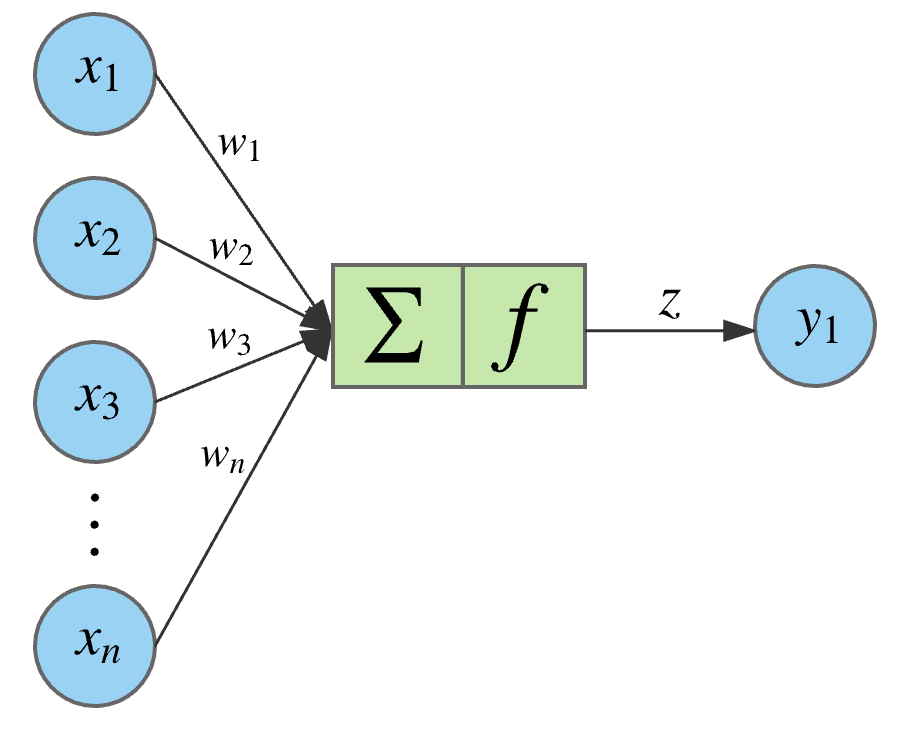
\includegraphics[width=0.6\textwidth]{neuron}
	\caption*{Single Neuron - McCulloch–Pitts model [A. Dertat 2017].}
	\end{figure}
\end{frame}

\begin{frame}[fragile]{Activation Function}
   \begin{itemize}
      \item McCulloch–Pitts neuron model
      \begin{equation*}
      y = \sigma(w_1x_1+w_2x_2+...+w_nx_n)
      \end{equation*}
   \end{itemize}
   \begin{tabular}{c  c}
		Rectified Linear Unit (ReLU) &  Hyperbolic Tangent (tanh) \vspace{10pt} \\ 
		$\sigma(x) = x^+ = \max(0,x)$ & $\sigma(x) = \frac{e^x-e^{-x}}{e^x+e^{-x}} = \tanh(x)$ \\ 
			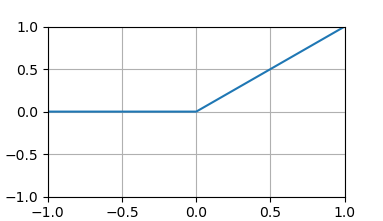
\includegraphics[width=.5\textwidth]{relu} &  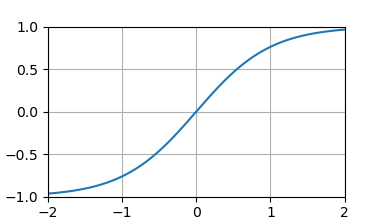
\includegraphics[width=.5\textwidth]{tanh}
			
   \end{tabular}

\end{frame}

\begin{frame}[fragile]{Neural Network}
   \begin{figure}
	\centering
	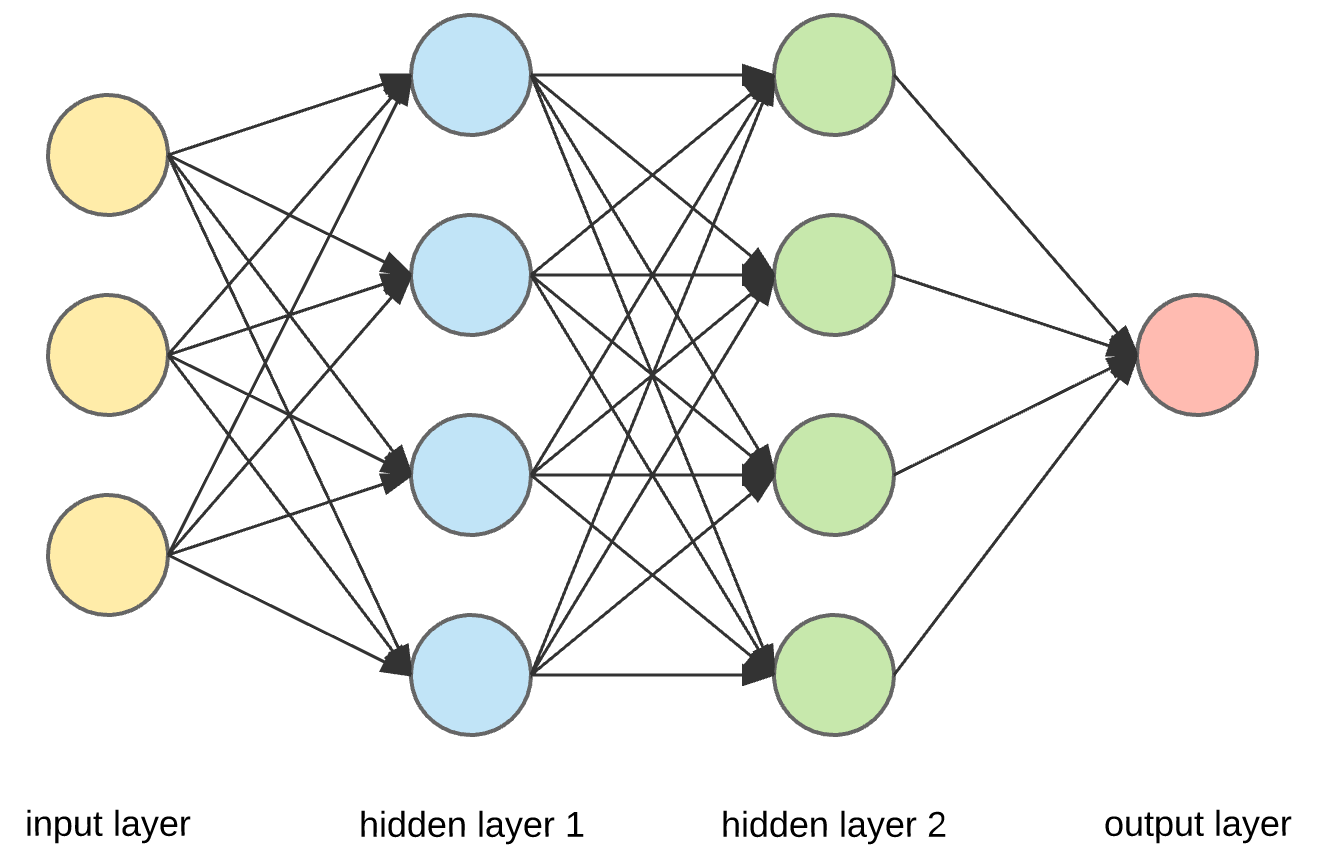
\includegraphics[width=0.7\textwidth]{network}
	\caption*{Feedforward Deep Neural Network [A. Dertat 2017].}
	\end{figure}
\end{frame}


\begin{frame}[fragile]{Neural Network Training}
   \begin{itemize}
      \item Function definition of network with $L$ layers
      \begin{equation*}
         f_W(x) = W_L\sigma(W_{L-1}\sigma(...W_1\sigma(W_0x)...))
      \end{equation*}
      \item Function application \& matrix multiplication
      \item Training = unconstrained optimization problem over training set:
      \begin{equation*}
      \begin{aligned}
      & \underset{W}{\text{minimize}}
      & C(W) &= \frac{1}{N}\sum\limits_{j=0}^{N}l(f_W(x_j)-y_j) \\
      \end{aligned}
      \end{equation*}
      \item $f_W(x_j)$ : prediction of network for $x_j$
      \item compare network prediction to target output $y_j$
      \item Minimize average loss for loss function $l(\cdot,\cdot)$
      \item Proxy for performance metric $P$ defined over the test set
   \end{itemize}
\end{frame}

\begin{frame}[fragile]{Gradient Descent}
	\begin{itemize}
		\item Training problem is solved using Gradient Descent:
      	\begin{equation*}
      		W_{k+1} = W_{k} - \eta_k\nabla C(W_k)
      	\end{equation*}
      	\begin{itemize}
      	\item $\eta_k$: step size a.k.a. "learning rate"
      	\item Gradient is calculated using Backpropagation algorithm
      	\end{itemize}
      	\item Cumbersome to calculate full gradient for large datasets
      	\begin{itemize}
      	\item $\Rightarrow$ Approximate gradient over "mini-batch" of datapoints
      	\item Stochastic Gradient Descent
      	\end{itemize}
      	\item Current best algorithms use adaptive learning rates
      	\begin{itemize}
      		\item AdaGrad, Rmsprop, ADAM, ...
      	\end{itemize}
      	\item Halting based on "early stopping" criterion
      	\begin{itemize}
      		\item $\Leftrightarrow$ pure optimization halts on small gradient 
      	\end{itemize}
      	
	
	\end{itemize}
\end{frame}

\begin{frame}[fragile]{Local Minima}
	\begin{itemize}
		\item Gradient Descent is a locally converging algorithm
		\item Cost function will have highly non-convex surface
		\item Possibly uncountably many local minima
		\item Finding global minimum is intractible
		\begin{itemize}
			\item "bad" local minima: have comparatively high cost value
			\item Hard to define exactly
		\end{itemize}
		\item " ... but experts now suspect that,
for sufficiently large neural networks, most local minima have a low cost function
value ... " [Goodfellow et. al. 2016]
		\item Other optimization challenges
		\begin{itemize}
			\item Ill-conditioned Hessian matrix
			\item Exploding/Vanishing gradients
			\item "Dying" ReLU
		\end{itemize}
	\end{itemize}
\end{frame}





\begin{frame}[fragile]{Neural networks as Dynamical Systems}
\begin{equation*}
	\begin{aligned}
	z_0 &= x \\
	z_{k+1} &= \sigma_k(W_kz_k), & k = 0,...,L \\
	f_W(x) &= z_{L+1} \\
	\end{aligned}
\label{st-eq}
\end{equation*}
\begin{itemize}
	\item Neural networks are dynamical systems
	\begin{itemize}
		\item Each layer is a state
	\end{itemize}
	\item Optimal Control objective  cost function:
	\begin{equation*}
		E(\theta) = \sum\limits_{s=1}^{L-1}g^s(a^s,\theta^s) + h(a^L)
	\end{equation*}
	\item NN training only considers terminal cost
\end{itemize}

\end{frame}
\begin{frame}[fragile]{Training as Optimal Control Problem}
\begin{equation*}
	\begin{aligned}
	& \underset{W,z}{\text{minimize}}
	& & \sum\limits_{j=0}^{n}||\sigma_L(W_Lz_L) - y_j||^2_2 \\
	& \text{subject to}
	& & z_{1,j} = \sigma_0(W_0,x_j), &j = 1,\ldots,n \\
	& & & z_{k+1,j} = \sigma_k(W_kz_{k,j}), &k = 1,\ldots,L-1,j = 1,\ldots,n
	\end{aligned}
	\label{ocp-eq}
\end{equation*}
\begin{table}
\centering
	\begin{tabular}{ c | c }
	Optimal Control & Neural Network\\ \hline
	decision variables & weight parameters\\
	state variables & (neuron) activation\\
	stage & layer \\
	\end{tabular}
\end{table}
\end{frame}

\note{MSE loss function, $n$ parellel systems, concatenated through the loss function, constrained non-linear program}

\begin{frame}[fragile]{Goal of the thesis: Solving the OCP}
\begin{itemize}
	\item Optimal control theory: two direct approaches
	\item Sequential Approach
	\begin{itemize}
		\item Direct Single Shooting
		\item Eliminate states using dynamics
		\item Reduces to unconstrained problem
		\item Small, highly nonlinear NLP
		\item Equivalent to backpropagation for NN [Dreyfus et al. 1990]
	\end{itemize}
	\item Simultaneous Approach
	\begin{itemize}
		\item Direct Multiple Shooting
		\item Keep states as variables
		\item Large, structured problem
		\item Novel approach for NN
		\item Topic of this thesis
	\end{itemize}
\end{itemize}
\end{frame}

\section{Multiple Shooting in MATLAB}

\begin{frame}[fragile]{Multiple Shooting in MATLAB}
\begin{itemize}
	\item Multiple shooting increases dimension of problem
	\begin{itemize}
		\item For network of width W, depth L, N datapoints:
		\item Single shooting: $\mathcal{O}(W^2L)$ variables
		\item Multiple shooting: $\mathcal{O}(W^2L + WLN)$ variables
	\end{itemize}
	\item Exploration of the multiple shooting approach
	\begin{itemize}
		\item Implemented in MATLAB
		\item Constrained NLP solved by \texttt{fmincon}
		\item Comparison with \texttt{nntoolbox}
		\item Training algorithm is \texttt{traingd}
	\end{itemize}
	\begin{table}
	\footnotesize
	\centering
	\hspace{-20pt}
	\begin{tabular}{r | c c | c c }
		& \multicolumn{2}{|c}{$\tanh$} & \multicolumn{2}{|c}{ReLU} \\
		Algorithm &avg tr MSE &avg run time & avg tr MSE & avg run time \\ \hline
		Gradient Descent & 0.0299 & 1.577s  & 0.0274 & 1.480s\\
		Multiple Shooting & 0.2350 & 23.82s & 0.2111 & 115.8s \\
	\end{tabular}
	\end{table}
\end{itemize}
\end{frame}

\begin{frame}[fragile]{Gradient Descent vs Multiple Shooting}
\begin{figure}
     \centering
     \begin{subfigure}[b]{0.45\textwidth}
         \centering
         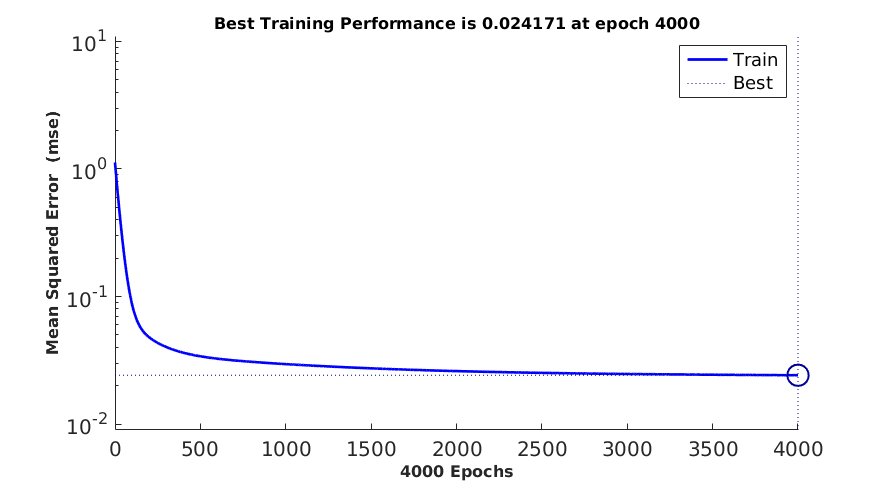
\includegraphics[width=\textwidth]{gdtrain}
         \caption*{\footnotesize Gradient Descent Training History}
         \label{gdtrain}
     \end{subfigure}
     \begin{subfigure}[b]{0.45\textwidth}
         \centering
         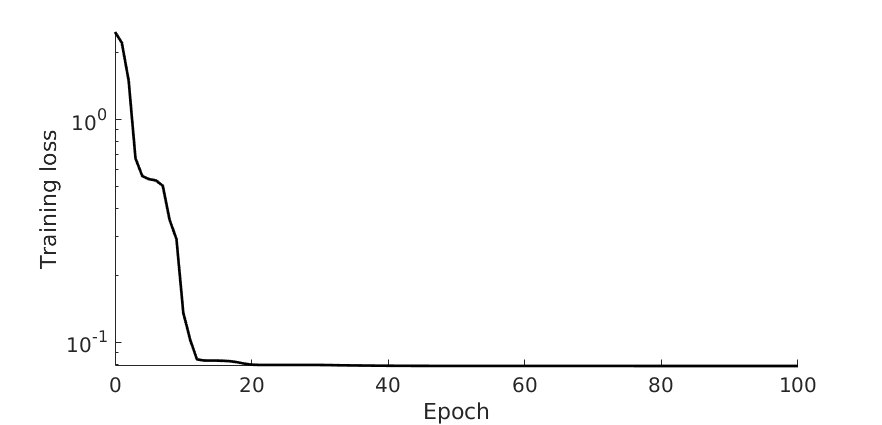
\includegraphics[width=\textwidth]{fmintrain}
         \caption*{\footnotesize Multiple Shooting Training History}
         \label{fmintrain}
     \end{subfigure}
     \begin{subfigure}[b]{0.49\textwidth}
         \centering
         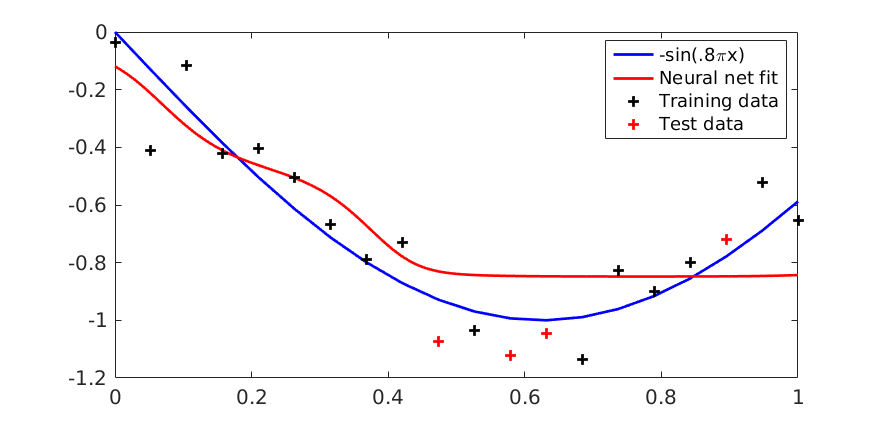
\includegraphics[width=\textwidth]{gdfit}
         \caption*{\footnotesize NN fit with Gradient Descent}
         \label{gdfit}
     \end{subfigure}
     \begin{subfigure}[b]{0.49\textwidth}
         \centering
         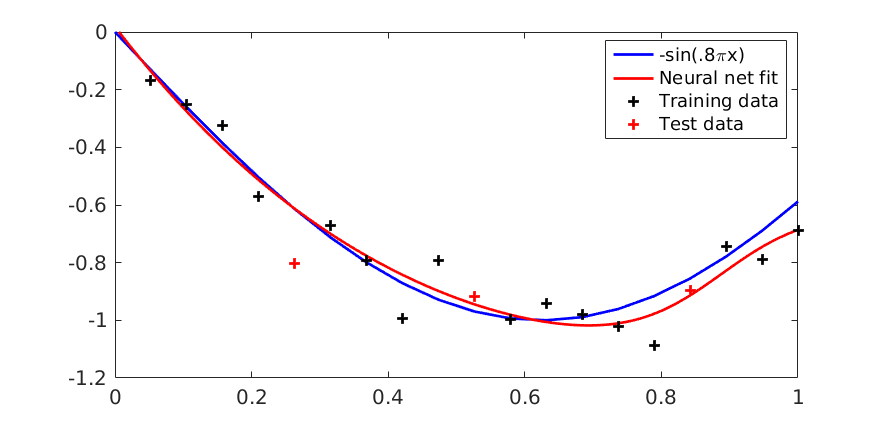
\includegraphics[width=\textwidth]{fminfit}
         \caption*{\footnotesize NN fit with Multiple Shooting}
         \label{fminfit}
     \end{subfigure}
    \caption*{Comparing algorithm performance for regression problem}
    \label{compalg}
\end{figure}
\end{frame}

\section{Augmented Lagrangian Method}

\begin{frame}[fragile]{Augmented Lagrangian Method}
\begin{itemize}
	\item \texttt{fmincon} not well suited for this problem
	\begin{itemize}
		\item $\Rightarrow$ implement specialized algorithm
		\item exploit structure in problem
	\end{itemize}
	\item Augmented Lagrangian Method
	\begin{itemize}
		\item Algorithmic framework for constrained NLP
		\item Similar to penalty method
	\end{itemize}
	\item Constrained NLP:
	\begin{equation*}
		\begin{aligned}
		& \underset{u}{\text{min}} & f(u) & \\
		& \text{s.t.} & h(u) &= 0 \\
		\end{aligned}
	\end{equation*}
\end{itemize}
\end{frame}

\begin{frame}[fragile]{Classical Augmented Lagrangian Method}
\begin{itemize}
	\item $\beta$-augmented Lagrangian:
	\begin{equation*}
		\underset{u}{\text{min}} \hspace{.5em} \underset{\lambda}{\text{max}} \hspace{.5em}  \mathcal{L}_\beta(u,\lambda) = f(u) + \langle\lambda,h(u)\rangle + \frac{\beta}{2} || h(u) ||^2_2
	\end{equation*}
	\item Converges to local minimizer of constrained problem if
	\begin{itemize}
		\item $\beta$ is large
		\item $\lambda$ is close to $\lambda^*$
	\end{itemize}
	\item Algorithm solves series of unconstrained problems
	\begin{gather*}
		u_{k+1} = \underset{u}{\text{argmin}} \hspace{.5em} \mathcal{L}_{\beta_k}(u,\lambda_k) \\
		\lambda_{k+1} = \lambda_k + \sigma_k h(u_{k+1})
	\end{gather*}
\end{itemize}
\end{frame}

\begin{frame}[fragile]{Classical Augmented Lagrangian Method}
\begin{itemize}
	\item Penalty parameter increases or is kept the same in each iteration
	\begin{itemize}
		\item depends on constraint violation
	\end{itemize}
	\item Stopping criterion:
	\begin{equation*}
		||h(u_k)|| \leq \tau_1 \hspace{.5em}\text{and}\hspace{.5em} ||\nabla_u\mathcal{L}_{\beta_k}(u_k,\lambda_k)|| \leq \tau_2
	\end{equation*}
	\item NN training has nonconvex $f$ with nonlinear constraints, inexact solution to inner problem
	\item Textbook theory requires strong assumptions, exact solution \relax
    \item Sahin et al. (2019) proposes alternative framework:
	\begin{itemize}
		\item Promises $\mathcal{\tilde{O}}(1/\epsilon^3)$ calls to first-order solver
		\item Theoretical estimates on convergence
	\end{itemize}
\end{itemize}
\end{frame}

\begin{frame}[fragile]{$\beta$-Augmented Lagrangian}
	\begin{equation*}
	\begin{aligned}
	& \underset{W,z}{\text{minimize}}
	& & \sum\limits_{j=0}^{n}||\sigma_L(W_Lz_L) - y_j||^2_2 
	& & & \underset{u}{\text{min}}
	& & \frac{1}{2} ||F(u)||^2_2 \\
	& \text{subject to}
	& & z_{1,j} = \sigma_0(W_0,x_j)  
	& \Leftrightarrow & & \text{s. t.} & &  h(u) = 0\\
	& & & z_{k+1,j} = \sigma_k(W_kz_{k,j}) \\
	\end{aligned}
\end{equation*}
\begin{itemize}
\item $u = \{W,z\}$ collects weight and state variables in single vector
\item minimizing $\beta$-Augmented Lagrangian is LS problem
\end{itemize}

\begin{equation}
	\begin{aligned}
	 & \underset{u}{\text{argmin}} & \mathcal{L}_{\beta}(u,\lambda) 
	     &= \frac{1}{2} ||F(u)||^2_2 + \langle\lambda,h(u)\rangle + \frac{\beta}{2} || h(u) ||^2_2 \\
	 & & &= \frac{\beta}{2} \Big|\Big|
		\begin{bmatrix}
			F(u)/\sqrt{\beta} \\
			h(u) + \lambda/\beta
		\end{bmatrix} \Big|\Big|^2_2 \\
	\end{aligned}
	\label{loss}
\end{equation}
\end{frame}



\begin{frame}[fragile]{Applied Augmented Lagrangian Method}
\begin{algorithm}[H]
\setstretch{1.2}
\SetAlgoLined
\SetKw{Kw}{Initialization}
\SetKwComment{Comment}{}{}
\SetCommentSty{emph}
\KwIn{Initial weights vector $W$, penalty parameter $\beta$, stopping tolerance $\tau$, input-target pairs $(x_i,y_i), i = 1,\ldots,n$}
\Kw{$u_0 = \{W,f_{W}(x)\}, \lambda_0 \in \mathcal{N}(0,1)$}
\Comment*[r]{Initialize state}
\For{k = 0,1,...}{
 	$\eta_k = 1/\beta^k$
 	\Comment*[r]{Update tolerance}
 	find $u_{k+1}$ such that \\
 	\Indp$||\nabla_{u_k}\mathcal{L}_{\beta^k}(u_k,\lambda_k)|| \leq \eta_k$ \label{ls-prob}
 	\Comment*[r]{Approx. primal solution}
 	\Indm$\sigma_{k+1} = \text{min}\big(\frac{||h(u_0)||\log^22}{||h(u_{k+1})||k \log^2(k+1)},1\big)$
 	\Comment*[r]{Update dual step size}
 	$\lambda_{k+1} = \lambda_k + \sigma_{k+1}h(u_{k+1})$
 	\Comment*[r]{Update dual variables}
 	
 	If $||\nabla_{u_{k+1}}\mathcal{L}_{\beta^k}(u_{k+1},\lambda_k)|| + ||h(u_{k+1})||<\tau$: \\
 	\Indp break
 	\Comment*[r]{Stopping Criterion}
 	
 }
 \label{algo}
\end{algorithm}
\end{frame}


\begin{frame}[fragile]{Convergence}
\begin{figure}
	\centering
	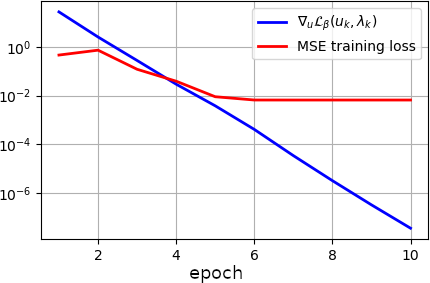
\includegraphics[width=.7\textwidth]{nabla}
	\caption*{Typical convergence behaviour of Algorithm \ref{algo}}
	\label{nabla}
\end{figure}
\end{frame}


\begin{frame}[fragile]{Jacobian}
	\begin{itemize}
		\item Inner problem is nonlinear least squares
		\begin{itemize}
			\item Solved using Trust Region Reflective method
			\item \texttt{scipy.optimize.least\_squares}
			\item Works best with analytical solution for Jacobian matrix
		\end{itemize}
		\item Jacobian matrix
		\begin{itemize}
			\item Dimension $\approx (DWN \times DW(N+W))$
			\item Sparse, banded structure
		\end{itemize}
		\item Numerical Verification
		\begin{itemize}
			\item Automatic differentiation
			\item \texttt{AlgoPy} library
			\item Confirms correctness of analytical solution
		\end{itemize}
	\end{itemize}
\end{frame}
\note{Every layer only connected to prev and next layer}

\begin{frame}[fragile]{Jacobian Derivation}
\begin{equation*}
M_{\beta}(u,\lambda) := \begin{bmatrix} F(u)/\sqrt{\beta} \\ h(u) + \lambda/\beta \end{bmatrix}, 
J_{M_{\beta}} := 
\begin{bmatrix}
\frac{\partial{M_{\beta}}}{\partial u_1} & 
\frac{\partial{M_{\beta}}}{\partial u_2} & ... & 
\frac{\partial{M_{\beta}}}{\partial u_n} \\
\end{bmatrix}
\end{equation*}
\begin{equation*}
	\begin{aligned}
	\frac{\partial{M_{\beta}}}{\partial W_k} &= -z_{k,j}\sigma'_k(W_kz_{k,j}) &, j = 1,\ldots,n, k = 0,\ldots,L \\
 	\frac{\partial{M_{\beta}}}{\partial z_k} &= \begin{bmatrix} 1 \\ -W_k\sigma'_k(W_kz_k) \end{bmatrix} &, k = 1,\ldots,L
 	\end{aligned}
 \end{equation*}
\begin{itemize}
	\item $W_k,z_k$ are matrices $\rightarrow$ derivatives are tensors
	\item $W_k,z_k$ vectorized $\rightarrow$ derivatives are block matrices
\end{itemize}
\end{frame}

\begin{frame}[fragile]{Visualisation of Jacobian}
	\begin{figure}
	  \centering
	  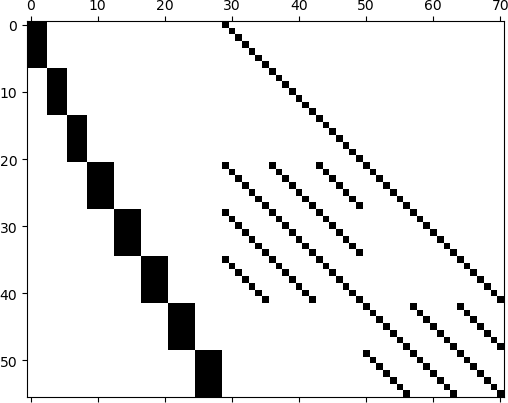
\includegraphics[width=.7\textwidth]{jac1.png} \\
	  \caption*{Network has 2 layers, 3 nodes/layer,  2 inputs, 2 outputs and 7 datapoints.}
	  \end{figure}
\end{frame}

\section{Regression Experiment}


\begin{frame}[fragile]{Test setup}
	\begin{itemize}
		\item Regression problem
		\begin{itemize}
			\item Approximate:
			\begin{equation*}y = \sin(x^2), x \in [0,\pi]\end{equation*}
			\item Using fully connected feedforward network
		\end{itemize}
		\item ADAM optimizer for comparison
		\begin{itemize}
			\item ADaptive Moment Estimation
			\item Robust, industry standard optimizer
			\item Stochastic gradient descent with adaptive learning rate
		\end{itemize}
		\item 20 training runs per test configuration
		\begin{itemize}
			\item Same initial conditions each run
			\item Same data, noise, weight initialization
			\item Gradient estimation over full dataset in each epoch
		\end{itemize}
		\item Intel® Core™ i5-7300HQ CPU \@ 2.50GHz with 8Gi RAM
	\end{itemize}
\end{frame}

\begin{frame}[fragile]{Halting criterion}
	\begin{itemize}
		\item Nonconvex Optimization
			\begin{itemize}
				\item Local minimizer of cost function: small gradient
			\end{itemize}	
		\item Machine Learning
		\begin{itemize}
			\item "Early Stopping"
			\item Based on performance metric on validation set
		\end{itemize}
		\item Time based, epoch based halting
		\item Goal of thesis: local minima $\Rightarrow$ Halt at local minimum
		\begin{itemize}
			\item ADAM: 10 epochs without any improvement to cost function
			\item ALM: 1 epoch without significant improvement:
				\begin{equation*}
				(1+\epsilon)C(W_{k+1}) > C(W_k)
				\end{equation*}
			\item Halting based on gradient
			\item Discards influence of states, constraint violation
		\end{itemize}
	\end{itemize}
\end{frame}


\begin{frame}
\centering
\footnotesize
\makebox[\textwidth]{
\begin{tabular}{c c}
	Good convergence & Bad convergence \\	
    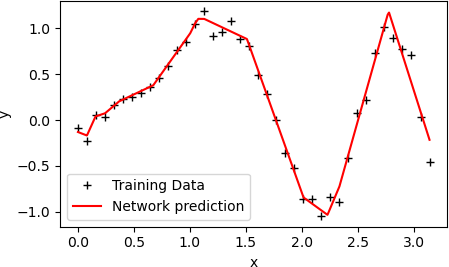
\includegraphics[width=.5\textwidth]{adamgood} &  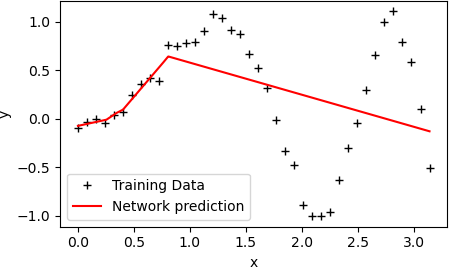
\includegraphics[width=.5\textwidth]{adambad} \\
	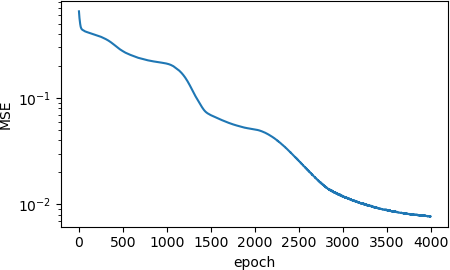
\includegraphics[width=.5\textwidth]{adamgoodconv} &  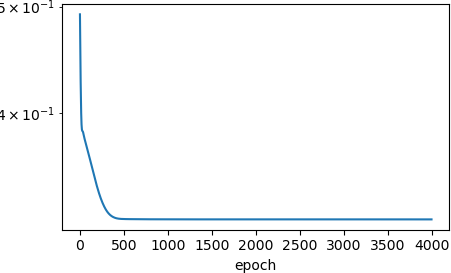
\includegraphics[width=.5\textwidth]{adambadconv} \\
\end{tabular}}
Examples of convergence behaviour of ADAM optimizer for a network using ReLU activation and 40 data points. The network has 2 hidden layers of 16 nodes.
\end{frame}

\begin{frame}
\centering
\footnotesize
\makebox[\textwidth]{
\begin{tabular}{c c}
	Good convergence & Convergence History \\	
    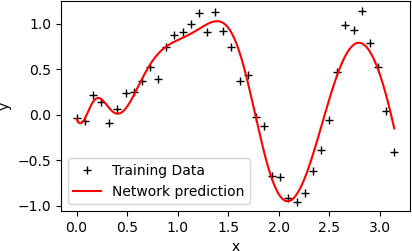
\includegraphics[width=.5\textwidth]{almgood} &  
    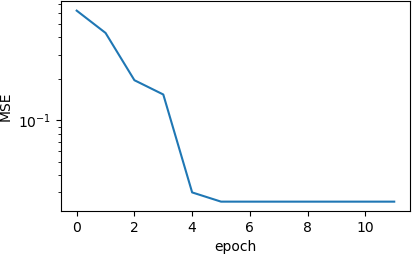
\includegraphics[width=.5\textwidth]{almgoodconv} \\
\end{tabular}}
Example of convergence behaviour of ALM optimizer for network using $tanh$ activation and 40 data points. The network has 2 hidden layers of 8 nodes.
\makebox[\textwidth]{
\begin{tabular}{c c}
	ADAM Histogram & ALM History \\	
    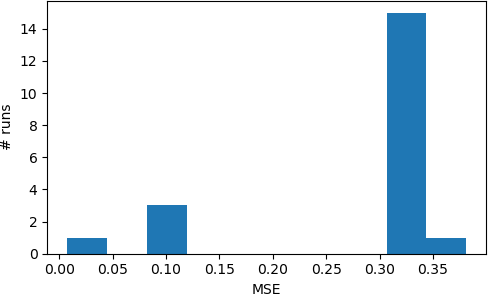
\includegraphics[width=.5\textwidth,height=.3\textheight]{hist} &  
    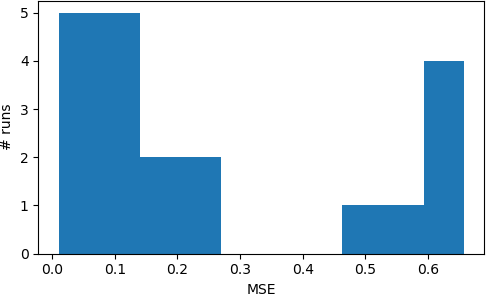
\includegraphics[width=.5\textwidth,height=.3\textheight]{almhist} \\
\end{tabular}}
MSE of  batch using 40 data points and ReLU activation function
\end{frame}

\begin{frame}[fragile]{Results for network with $\tanh$ activation}
\begin{table}
\renewcommand{\arraystretch}{1.3}
\centering
\small
\makebox[\textwidth][c]{
\begin{tabular}{r | r| c c c c c || r| c c c c c|}
\multicolumn{1}{c}{} & \multicolumn{6}{c}{$\sigma(\cdot) = \tanh(\cdot)$} \\ \cline{2-7}
        &                   N & avg MSE       & best MSE        & time(s)  & avg epochs   & $\frac{\text{converging runs}}{\text{20 runs}}$  \\ \cline{2-7}
    ADAM& \multirow{2}{*}{10} & $ 2.09e^{-2} $ & $1.20e^{-11} $ & $ 18.7 $ & $ 3790 $ & $ 17 $ \\
    ALM & 				      & $ 2.10e^{-1} $ & $ 1.59e^{-1} $ & $ 1.85 $ & $ 6.38 $ & $ 16 $ \\ \cline{2-7}
    ADAM& \multirow{2}{*}{20} & $ 1.25e^{-2} $ & $ 9.84e^{-4} $ & $ 19.8 $ & $ 3960 $ & $ 17 $ \\
    ALM & 					  & $ 5.87e^{-2} $ & $ 7.69e^{-3} $ & $ 8.06 $ & $ 7.50 $ & $ 20 $ \\ \cline{2-7}
    ADAM& \multirow{2}{*}{40} & $ 2.56e^{-2} $ & $ 7.58e^{-3} $ & $ 19.2 $ & $ 3920 $ & $ 15 $ \\
    ALM &                     & $ 1.61e^{-2} $ & $ 7.90e^{-3} $ & $ 11.6 $ & $ 6.90 $ & $ 20 $ \\ \cline{2-7}
\end{tabular}
}
\end{table}
\centering
Fully connected feedforward network, 2 hidden layers, 8 nodes / layer
\end{frame}

\begin{frame}[fragile]{Results for network with ReLU activation}
\centering
\begin{table}
\renewcommand{\arraystretch}{1.3}
\centering
\small
\makebox[\textwidth][c]{
\begin{tabular}{r | r| c c c c c |}
\multicolumn{1}{c}{} & \multicolumn{6}{c}{$\sigma(\cdot) = \max(\cdot,0)$} \\ \cline{2-7}
        &                   N & avg MSE        & best MSE       & time(s)  & avg epochs   & $\frac{\text{converging runs}}{\text{20 runs}}$   \\ \cline{2-7}
    ADAM& \multirow{2}{*}{20} & $ 1.22e^{-1} $ & $ 3.15e^{-3} $ & $ 30.3 $ & $ 3500 $ & $ 5  $ \\ 
    ALM & 				      & $ 1.63e^{-1} $ & $ 1.08e^{-2} $ & $ 4.41 $ & $ 5.47 $ & $ 15 $ \\ \cline{2-7}
    ADAM& \multirow{2}{*}{40} & $ 6.28e^{-2} $ & $ 8.85e^{-3} $ & $ 22.4 $ & $ 2690 $ & $ 5  $ \\ 
    ALM & 					  & $ 9.89e^{-2} $ & $ 1.37e^{-2} $ & $ 8.09 $ & $ 5.11 $ & $ 18 $ \\ \cline{2-7}
    ADAM& \multirow{2}{*}{80} & $ 7.61e^{-2} $ & $ 7.64e^{-3} $ & $ 29.9 $ & $ 3150 $ & $ 4  $ \\ 
    ALM &                     & $ 1.02e^{-1} $ & $ 1.03e^{-2} $ & $ 25.3 $ & $ 4.21 $ & $ 14 $ \\ \cline{2-7}
\end{tabular}
}
\end{table}
\centering
Fully connected feedforward network, 2 hidden layers, 16 nodes / layer
\end{frame}

\section{Timeseries Experiment}
\begin{frame}[fragile]{Santa Fe timeseries data}
   	\centering
	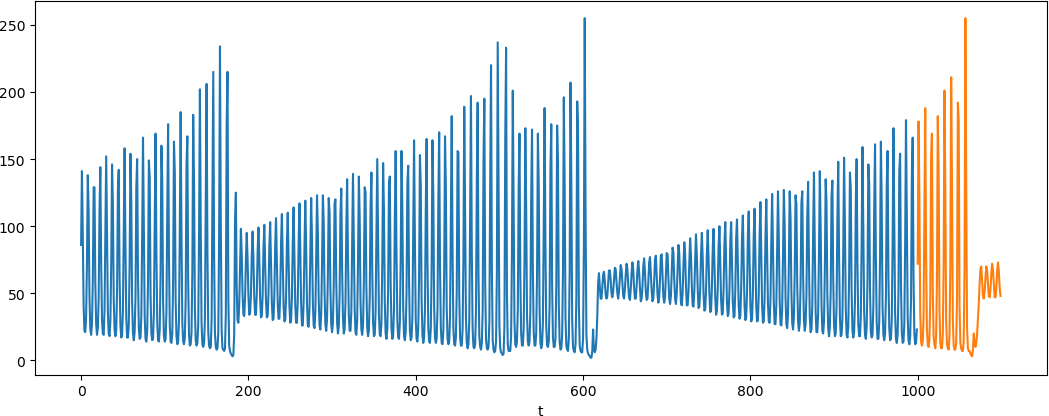
\includegraphics[width=\textwidth]{santafe}
	\begin{itemize}
		\item Far-infrared laser fluctuations, coupled nonlinear ODEs
		\item 1000 data points training, 100 points test data
	\end{itemize}
\end{frame}
\begin{frame}[fragile]{Test Setup}
	\begin{itemize}
		\item Approximate using recurrent neural network:
		\begin{equation*}
		\hat{y}_{k+1} = f_W(\begin{bmatrix} \hat{y}_{k} & \hat{y}_{k-1} & ... & \hat{y}_{k-p}\end{bmatrix}^T)
		\end{equation*}
		\item Previous predictions used to make next prediction
		\item $\tanh$ activation, 80 inputs, 1 layer, 48 nodes
		\item 920 training pairs, 600 in training set, 320 in validation set
		\item 4 training runs per algorithm, same initial conditions
		\item Intel® Core™ i5-7300HQ CPU \@ 2.50GHz with 8Gi RAM
	\end{itemize}
\end{frame}

\begin{frame}
\centering
\footnotesize
\makebox[\textwidth]{
\begin{tabular}{c c}	
    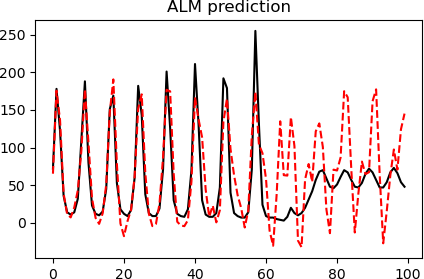
\includegraphics[width=.5\textwidth]{almpred} &  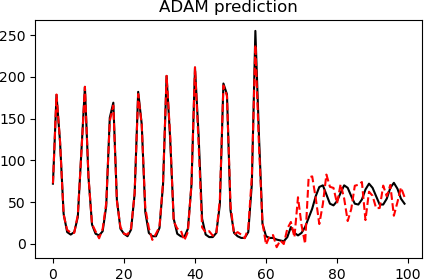
\includegraphics[width=.5\textwidth]{adampred} \\
	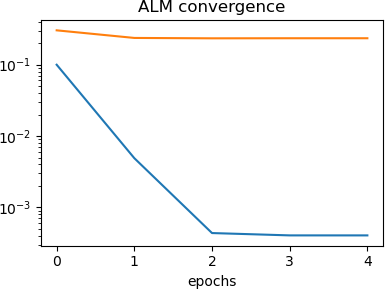
\includegraphics[width=.5\textwidth]{almlaserconv} &  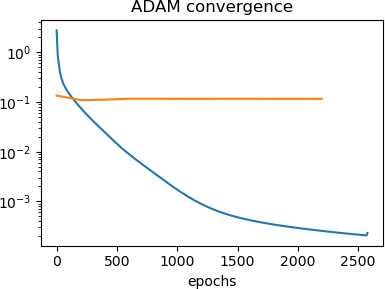
\includegraphics[width=.5\textwidth]{adamlaserconv} \\
\end{tabular}}
Test MSE in blue, Validation MSE in orange
\end{frame}

\begin{frame}[fragile]{Timeseries data test results}
\begin{table}
\renewcommand{\arraystretch}{1.3}
\centering
\footnotesize
\makebox[\textwidth]{
\begin{tabular}{r| c c c c c c }
	Algo & avg MSE          & best MSE         & avg pred MSE     & best pred MSE    & epochs   & time \\ \hline
     ALM & $ 3.712e^{-4} $ & $ 2.779e^{-4} $ & $ 1.070e^0    $ & $ 8.288e^{-1} $ & $ 5    $ & 1201s \\
    ADAM & $ 2.517e^{-4} $ & $ 2.329e^{-4} $ & $ 2.016e^{-1} $ & $ 9.100e^{-2} $ & $ 2353 $ & 20.9s
\end{tabular}}
\end{table}
\begin{itemize}
	\item ALM is very slow: 20min on avg, compared to 20s for ADAM
	\item Similar performance for training data, ADAM much better on test data
	\item Most calls to jacobian are in first epochs:
\end{itemize}
\begin{table}[h!]
\footnotesize
\centering
\begin{tabular}{r| c c c c c }
Epoch	 	& 1	& 2 & 3 & 4 & 5 \\ \hline
\#evals & 42.25 & 12.75 & 17.0  &   3.0  &    2.0 \\
\end{tabular}
\caption*{Average number of Jacobian evaluations per epoch}
\label{jevaltab}
\end{table}
\end{frame}

\section{Conclusion}

\begin{frame}[fragile]{Conclusion}
	\begin{itemize}
		\item Novel perspective on neural network training using control theory
		\begin{itemize}
			\item Single shooting: Backpropagation with Gradient Descent
			\item Multiple shooting: new algorithm
			\item MATLAB provides POC
		\end{itemize}
		\item ALM framework implemented
		\begin{itemize}
			\item Framework adapted from [Sahin et al. 2019]
			\item Analytical solution for Jacobian
		\end{itemize}
		\item Numerical Tests
		\begin{itemize}
			\item ALM outperforms ADAM for network with many bad local minima
			\item ALM becomes impractical for larger datasets
		\end{itemize}
		\item Mini-batch approach for ALM can mitigate scaling problem
		\begin{itemize}
			\item Cannot be easily adapted from stochastic gradient descent
			\item Multiple shooting is harder to warm-start
		\end{itemize}
	\end{itemize}
\end{frame}

\section*{References}
\begin{frame}[fragile]{References}
\footnotesize
\begin{tabular}{c p{.9\textwidth}}
[1] & A. Dertat. Applied deep learning - part 1: Artificial neural networks. URL: https://towardsdatascience.com/applied-deep-learning-part-1-artificial-neural-networks-d7834f67a4f6, retrieved 2021-05-31 \\\relax
[2] & S. E. Dreyfus. Artificial neural networks, back propagation, and the kelley-bryson gradient procedure. Journal of Guidance, Control, and Dynamics, 13(5):926–928, 1990. \\\relax
[3] & I. Goodfellow, Y. Bengio, and A. Courville. Deep Learning. MIT Press, 2016. URL: http://www.deeplearningbook.org. \\\relax
[4] & H. Li, Z. Xu, G. Taylor, C. Studer, and T. Goldstein. Visualizing the loss landscape of neural nets, 2018. \\\relax
[5] & M. F. Sahin, A. eftekhari, A. Alacaoglu, F. Latorre, and V. Cevher. An inexact augmented lagrangian framework for nonconvex optimization with nonlinear constraints. In H. Wallach, H. Larochelle, A. Beygelzimer, F. d'Alché-Buc, E. Fox, and R. Garnett, editors, Advances in Neural Information Processing Systems, volume 32. Curran Associates, Inc., 2019. \\\relax
\end{tabular}
\end{frame}



\begin{frame}[c,plain,noframenumbering]
\begin{tikzpicture}[remember picture,overlay]
\fill[fill=kul-blue]
    (current page.south east)  rectangle  ([shift={(0,-0.1\paperheight)}]current page.north west)   ;
\end{tikzpicture}

\centering
\textcolor{white}{Questions}
\end{frame}


\appendix
\begin{frame}[noframenumbering,label=extraframe]{Comparison to Evens et al (2021)}
\begin{itemize}
	\item Different ALM framework
	\item Gauss-Newton approach for inner problem
	\item Not tested on larger datasets
\end{itemize}
\end{frame}
\begin{frame}[noframenumbering,label=extraframe]{Loss Functions}
\renewcommand{\arraystretch}{2}
\centering
\begin{tabular}{ c c}
	quadratic loss function & cross-entropy loss \\
	$||y^2-\hat y^2||$ & $y\log(\hat y)+(1-y)\log(1-\hat y)$ \\
	Mean Squared Error(MSE) & negative log-likelihood \\
	Regression & Classification\\
\end{tabular}
\end{frame}

\begin{frame}[noframenumbering,label=extraframe] 
\centering
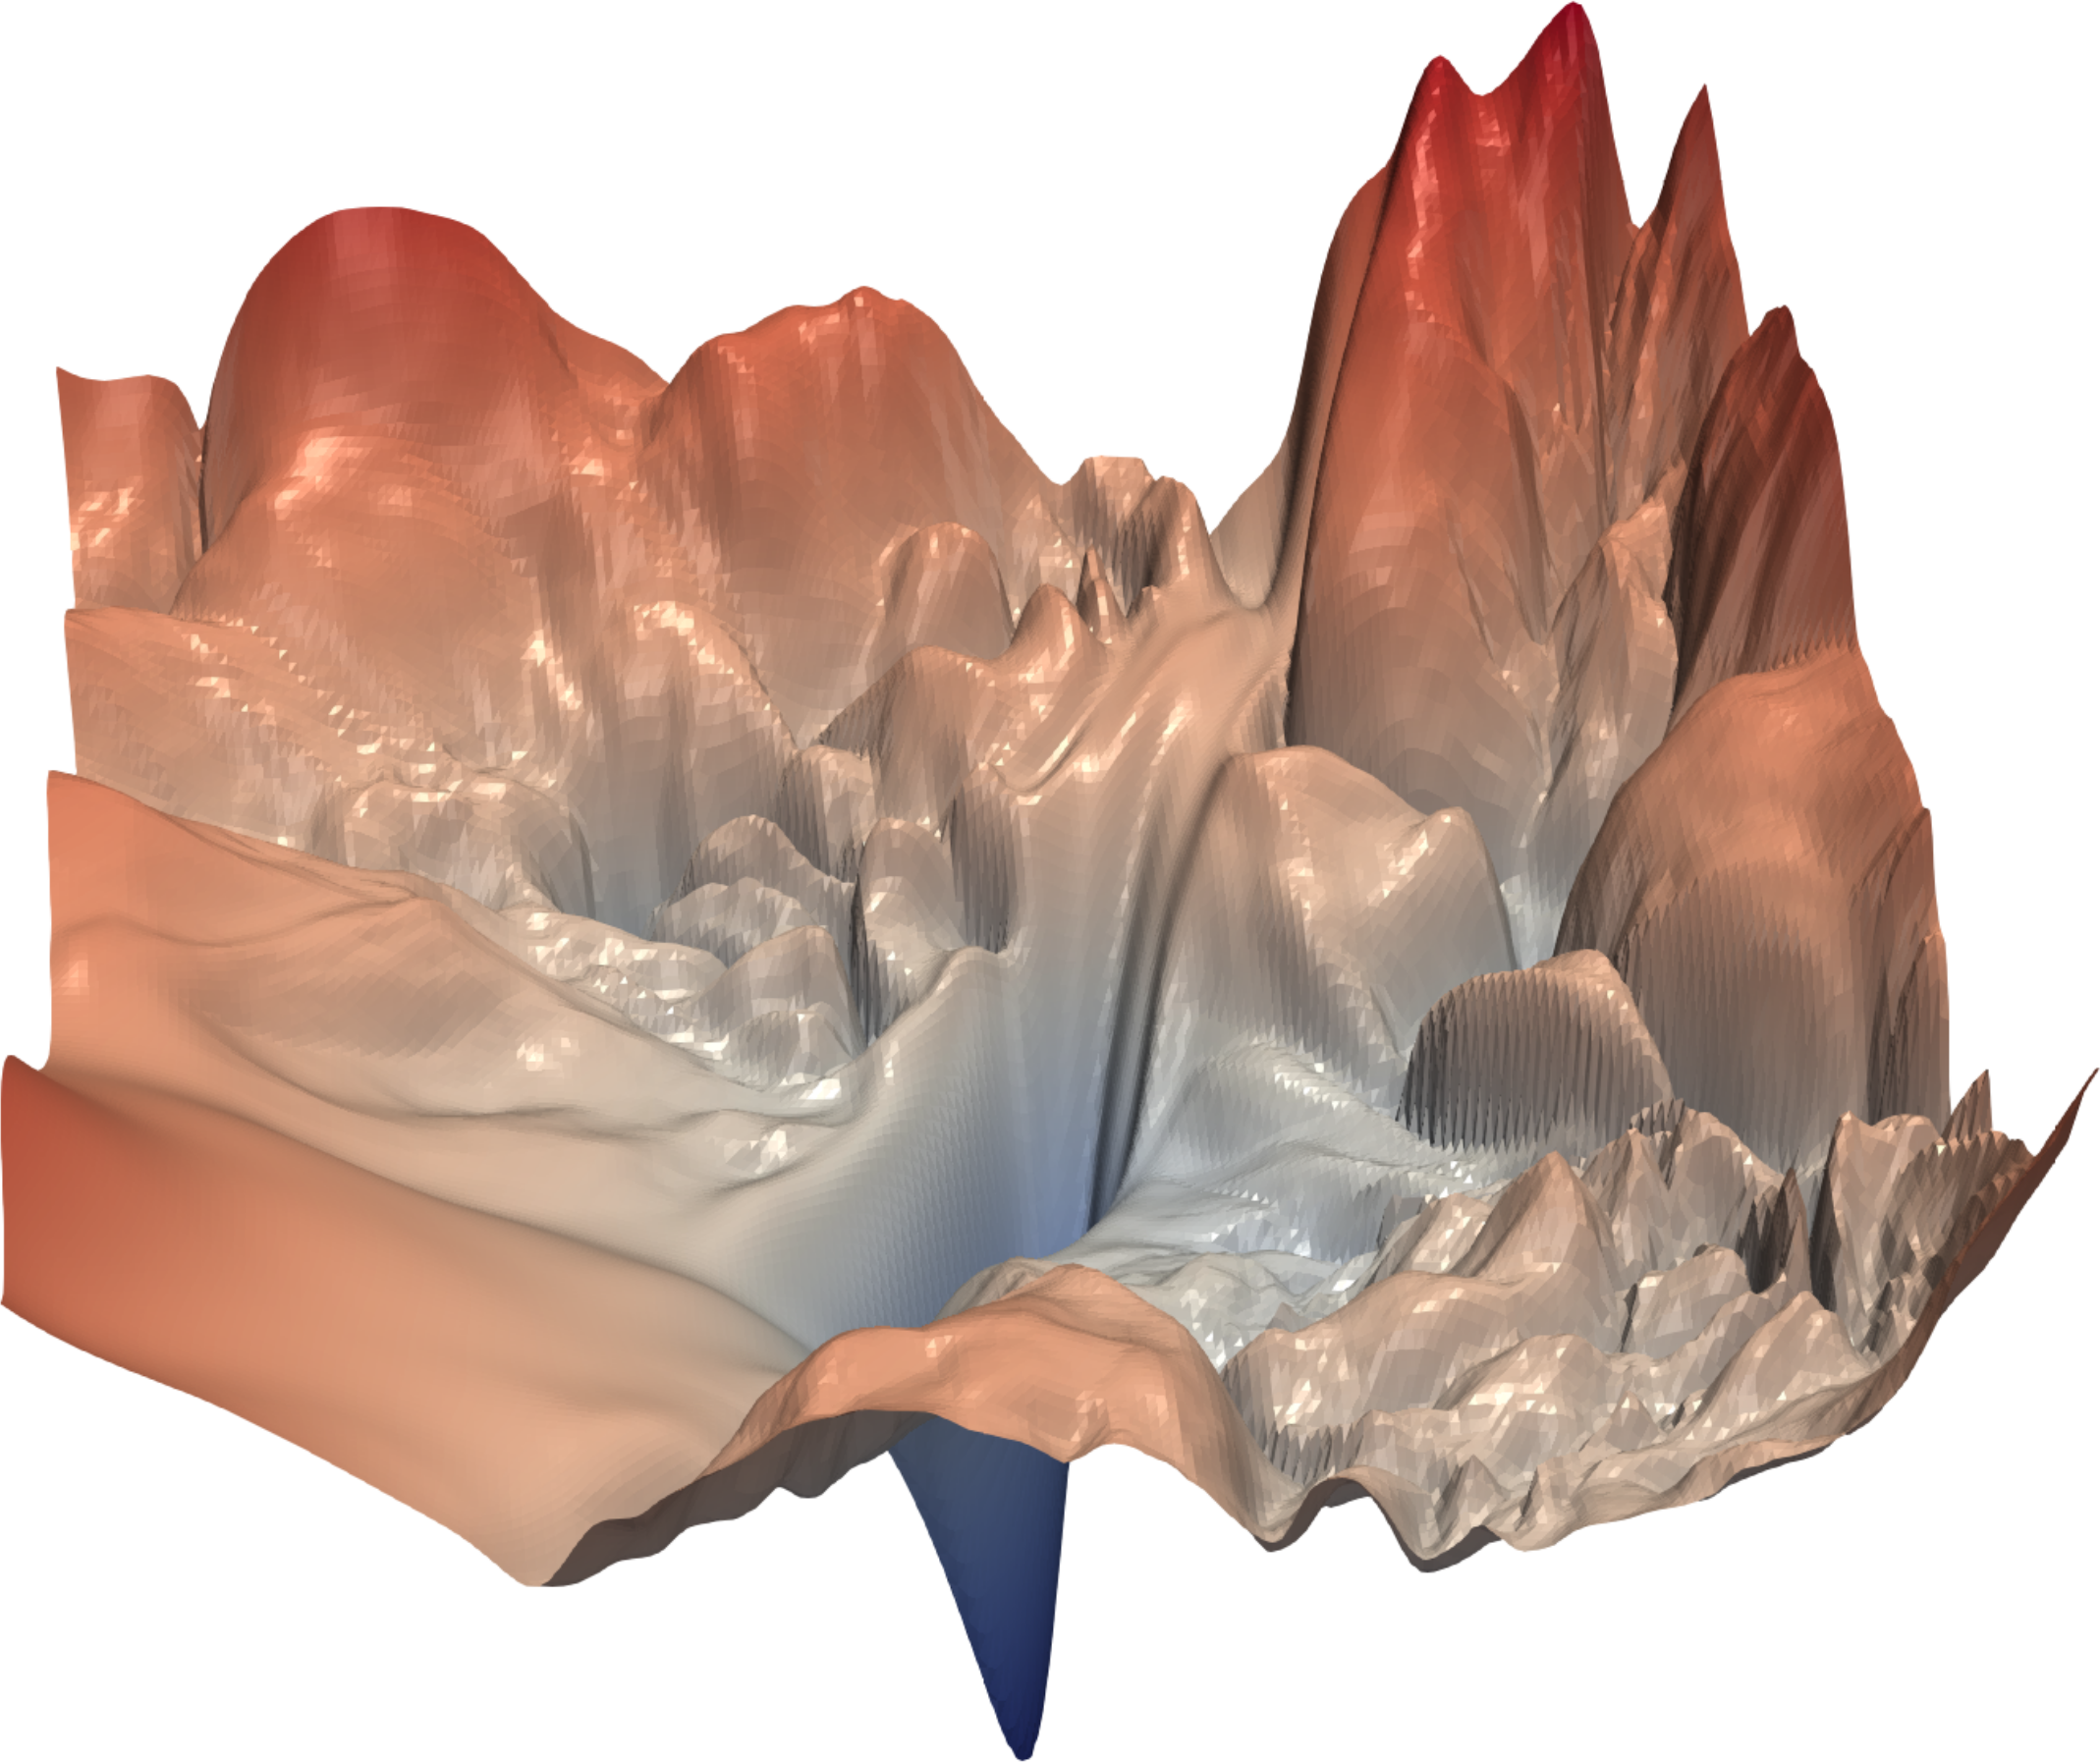
\includegraphics[width=.8\textwidth]{surface1}

Visualisation of loss surface of ResNet-56 [Li et al. 2018].
\end{frame}

\end{document}
